% ===================================================================
%  Week 10 — Session 1: Detecting distinctive points
% ===================================================================
\documentclass[10pt,aspectratio=169]{beamer}
% ===================================================================
%  Shared Beamer preamble for "Practical Image Processing"
%  English slides. Compile with pdfLaTeX.
% ===================================================================

\usetheme{metropolis}
\usepackage[T1]{fontenc}
\usepackage[utf8]{inputenc}
\usepackage{lmodern}
\usepackage{listings}
\usepackage{tcolorbox}
\usepackage{fontawesome5}
\usepackage{booktabs}
\usepackage{amsmath,amssymb}
\usepackage{tikz}
\usepackage{pgfplots}
\pgfplotsset{compat=1.17}
\usetikzlibrary{arrows.meta,positioning,shapes.geometric,fit,backgrounds,matrix}
\tcbuselibrary{skins,breakable}

% ---- Palette --------------------------------------------------------
\definecolor{coursePrimary}{HTML}{1B4965}   % deep blue
\definecolor{courseAccent}{HTML}{E76F51}    % coral
\definecolor{courseGood}{HTML}{2A9D8F}      % teal
\definecolor{courseBad}{HTML}{C0392B}       % red
\definecolor{courseInfo}{HTML}{2980B9}      % blue
\definecolor{codeBg}{HTML}{F5F6FA}
\definecolor{codeKw}{HTML}{8E44AD}
\definecolor{codeStr}{HTML}{2A9D8F}
\definecolor{codeCom}{HTML}{7F8C8D}

\setbeamercolor{frametitle}{bg=coursePrimary}
\setbeamercolor{progress bar}{fg=courseAccent}
\setbeamercolor{alerted text}{fg=courseAccent}
\metroset{block=fill,sectionpage=progressbar,numbering=fraction}

% ---- Code listings (Python is built into listings) -----------------
\lstdefinestyle{course}{
  backgroundcolor=\color{codeBg},
  basicstyle=\ttfamily\scriptsize,
  keywordstyle=\color{codeKw}\bfseries,
  stringstyle=\color{codeStr},
  commentstyle=\color{codeCom}\itshape,
  numberstyle=\tiny\color{codeCom},
  numbers=left, numbersep=6pt,
  showstringspaces=false, breaklines=true, breakatwhitespace=true,
  tabsize=4, columns=fullflexible,
  frame=single, framesep=4pt, rulecolor=\color{gray!30},
  keepspaces=true, upquote=true, language=Python,
}
\lstset{style=course}
\lstdefinelanguage{bash}{
  keywords={cd,pip,python,venv,source,import}, sensitive=true,
  morecomment=[l]{\#}, morestring=[b]', morestring=[b]",
}

% ---- Reusable callout boxes ----------------------------------------
\newtcolorbox{goodbox}[1][Good practice]{colback=courseGood!8,colframe=courseGood,
  fonttitle=\bfseries,title={\faCheck~#1},boxrule=0.6pt,left=4pt,right=4pt,top=3pt,bottom=3pt}
\newtcolorbox{badbox}[1][Pitfall]{colback=courseBad!8,colframe=courseBad,
  fonttitle=\bfseries,title={\faTimes~#1},boxrule=0.6pt,left=4pt,right=4pt,top=3pt,bottom=3pt}
\newtcolorbox{infobox}[1][Note]{colback=courseInfo!8,colframe=courseInfo,
  fonttitle=\bfseries,title={\faInfoCircle~#1},boxrule=0.6pt,left=4pt,right=4pt,top=3pt,bottom=3pt}
\newtcolorbox{mathbox}[1][Math]{colback=coursePrimary!6,colframe=coursePrimary,
  fonttitle=\bfseries,title={\faCalculator~#1},boxrule=0.6pt,left=4pt,right=4pt,top=3pt,bottom=3pt}

\newcommand{\keyidea}[1]{\begin{alertblock}{Key idea}#1\end{alertblock}}
\newcommand{\term}[1]{\textbf{\color{coursePrimary}#1}}
\newcommand{\code}[1]{\lstinline[basicstyle=\ttfamily\small]|#1|}

% ---- A helper to draw a small pixel grid, cells shaded by value ----
% \pixelgrid{ {10,20,120,200,240}, {30,60,130,180,230}, ... }
\newcommand{\pixelgrid}[1]{%
  \begin{tikzpicture}[font=\scriptsize,scale=0.6]
    \foreach \row [count=\ry] in {#1} {
      \foreach \val [count=\cx] in \row {
        \draw[gray,fill=coursePrimary!8] (\cx,-\ry) rectangle ++(1,-1);
        \node at (\cx+0.5,-\ry-0.5) {\val};
      }
    }
  \end{tikzpicture}}


\title{Feature Detection \& Matching}
\subtitle{Week 10 — Session 1: Corners \& descriptors — finding distinctive points}
\author{Practical Image Processing}
\date{Lecture 10.1 \textbullet\ 60--70 min}

\begin{document}

\maketitle

\begin{frame}{Recap \& today}
  \begin{columns}[T]
    \begin{column}{0.58\textwidth}
      \begin{itemize}
        \item Wk5--9: edges, regions, shapes — describing an image's content.
        \item \alert{This session:} \term{features} — distinctive points (corners) and how to
              turn each into a \term{descriptor} vector.
        \item Next session: \term{matching} those descriptors across images and rejecting bad matches.
      \end{itemize}
    \end{column}
    \begin{column}{0.42\textwidth}
      \begin{alertblock}{DocScan milestone}
        Finding repeatable points on a photographed page is the first step to aligning it to a
        template — the setup for Week 11's perspective correction.
      \end{alertblock}
    \end{column}
  \end{columns}
\end{frame}

\begin{frame}{Roadmap — Session 1}\tableofcontents\end{frame}

% ==================================================================
\section{What makes a good feature}
% ==================================================================

\begin{frame}{What is a good feature point?}
  \begin{itemize}
    \item \term{Distinctive}: it looks different from its surroundings (so it can be found again).
    \item \term{Repeatable}: the same physical point is detected across images (different view/light).
    \item \term{Local}: described by a small patch, robust to partial occlusion.
  \end{itemize}
  \keyidea{Flat regions and straight edges are ambiguous; \term{corners} are the classic good feature — they pin down a location in 2D.}
\end{frame}

\begin{frame}{Flat / edge / corner — the intuition}
  \begin{columns}[T]
    \begin{column}{0.52\textwidth}
      \begin{itemize}
        \item \term{Flat}: slide the window anywhere $\rightarrow$ patch unchanged $\rightarrow$ no localization.
        \item \term{Edge}: slide \emph{along} the edge $\rightarrow$ unchanged $\rightarrow$ 1D ambiguity.
        \item \term{Corner}: slide \emph{any} direction $\rightarrow$ patch changes $\rightarrow$ pinned in 2D.
      \end{itemize}
    \end{column}
    \begin{column}{0.48\textwidth}
      \begin{center}
      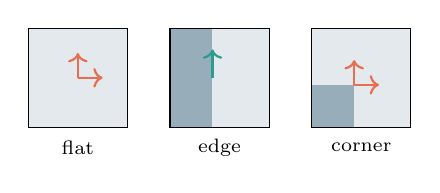
\begin{tikzpicture}[scale=0.9,font=\scriptsize]
        % flat
        \fill[coursePrimary!12] (0,0) rectangle (1.4,1.4);
        \draw (0,0) rectangle (1.4,1.4);
        \draw[courseAccent,thick,->] (0.7,0.7)--(1.05,0.7);
        \draw[courseAccent,thick,->] (0.7,0.7)--(0.7,1.05);
        \node at (0.7,-0.28) {flat};
        % edge
        \begin{scope}[xshift=2.0cm]
          \fill[coursePrimary!12] (0,0) rectangle (1.4,1.4);
          \fill[coursePrimary!45] (0,0) rectangle (0.6,1.4);
          \draw (0,0) rectangle (1.4,1.4);
          \draw[courseGood,thick,->] (0.6,0.7)--(0.6,1.1);
          \node at (0.7,-0.28) {edge};
        \end{scope}
        % corner
        \begin{scope}[xshift=4.0cm]
          \fill[coursePrimary!12] (0,0) rectangle (1.4,1.4);
          \fill[coursePrimary!45] (0,0) rectangle (0.6,0.6);
          \draw (0,0) rectangle (1.4,1.4);
          \draw[courseAccent,thick,->] (0.6,0.6)--(0.95,0.6);
          \draw[courseAccent,thick,->] (0.6,0.6)--(0.6,0.95);
          \node at (0.7,-0.28) {corner};
        \end{scope}
      \end{tikzpicture}
      \end{center}
    \end{column}
  \end{columns}
  \vspace{2pt}
  \begin{mathbox}
    The \term{Harris} detector turns ``does the patch change if I shift it?'' into linear algebra
    on the image gradients.
  \end{mathbox}
\end{frame}

\begin{frame}{The sliding-window energy}
  \begin{itemize}
    \item Shift a window by $(u,v)$ and measure how much the patch changes:
    \[ E(u,v)=\sum_{(x,y)\in W} w(x,y)\,\big[I(x+u,y+v)-I(x,y)\big]^2 . \]
    \item First-order Taylor: $I(x+u,y+v)\approx I(x,y)+I_x u + I_y v$, so
    \[ E(u,v)\approx \begin{bmatrix} u & v \end{bmatrix} \, M \, \begin{bmatrix} u \\ v \end{bmatrix},
       \qquad M=\sum_W w\begin{bmatrix} I_x^2 & I_xI_y \\ I_xI_y & I_y^2 \end{bmatrix}. \]
  \end{itemize}
  \keyidea{The change energy is a quadratic form in the shift. The matrix $M$ (the \term{structure matrix}) encodes all directions at once.}
\end{frame}

% ==================================================================
\section{The Harris corner detector}
% ==================================================================

\begin{frame}{The structure matrix, intuitively}
  \begin{itemize}
    \item Look at how image gradients $(I_x, I_y)$ vary inside a small window.
    \item The two eigenvalues $\lambda_1,\lambda_2$ of $M$ say how much the patch changes in the two
          principal directions.
  \end{itemize}
  \begin{center}
  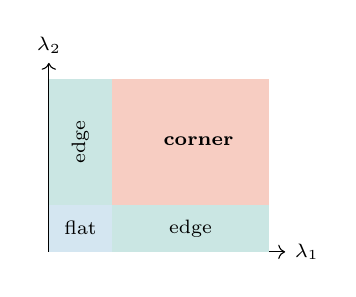
\begin{tikzpicture}[font=\scriptsize]
    \draw[->] (0,0)--(3,0) node[right]{$\lambda_1$};
    \draw[->] (0,0)--(0,2.4) node[above]{$\lambda_2$};
    \fill[courseInfo!20] (0,0) rectangle (0.8,0.6);
    \node at (0.4,0.3) {flat};
    \fill[courseGood!25] (0.8,0) rectangle (2.8,0.6);
    \node at (1.8,0.3) {edge};
    \fill[courseGood!25] (0,0.6) rectangle (0.8,2.2);
    \node[rotate=90] at (0.4,1.4) {edge};
    \fill[courseAccent!35] (0.8,0.6) rectangle (2.8,2.2);
    \node at (1.9,1.4) {\textbf{corner}};
  \end{tikzpicture}
  \end{center}
  \begin{mathbox}
    Both small $\rightarrow$ flat. One large $\rightarrow$ edge. \alert{Both large $\rightarrow$ corner.}
  \end{mathbox}
\end{frame}

\begin{frame}{Harris score — avoiding the eigenvalues}
  \begin{itemize}
    \item Computing $\lambda_1,\lambda_2$ per pixel is costly. Harris uses determinant and trace instead:
    \[ R=\det(M)-k\,\big[\mathrm{tr}(M)\big]^2
        = \lambda_1\lambda_2 - k(\lambda_1+\lambda_2)^2, \quad k\approx0.04\text{--}0.06. \]
    \item $R$ large positive $\rightarrow$ corner. $R<0 \rightarrow$ edge. $|R|$ small $\rightarrow$ flat.
  \end{itemize}
  \begin{mathbox}
    $\det(M)=I_x^2I_y^2-(I_xI_y)^2$ and $\mathrm{tr}(M)=I_x^2+I_y^2$ (summed over the window) — both
    are cheap to accumulate.
  \end{mathbox}
\end{frame}

\begin{frame}{Worked example — the Harris score}
  Suppose over a window we summed:
  \[ \textstyle\sum I_x^2 = 5,\quad \sum I_y^2 = 4,\quad \sum I_xI_y = 1,\quad k=0.05. \]
  \begin{columns}[T]
    \begin{column}{0.5\textwidth}
      \begin{align*}
        \det(M) &= (5)(4)-(1)^2 = 19,\\
        \mathrm{tr}(M) &= 5+4 = 9,\\
        R &= 19 - 0.05\,(9)^2\\
          &= 19 - 4.05 = \mathbf{14.95}.
      \end{align*}
    \end{column}
    \begin{column}{0.5\textwidth}
      \begin{infobox}[Reading it]
        $R \gg 0$: both gradient directions are strong $\Rightarrow$ a \term{corner}. \\[3pt]
        Contrast: an edge with $\sum I_x^2=9,\ \sum I_y^2=0,\ \sum I_xI_y=0$ gives $\det=0$,
        $R=-0.05(81)=-4.05<0$.
      \end{infobox}
    \end{column}
  \end{columns}
\end{frame}

\begin{frame}{Harris corners — on a real car}
  \begin{columns}[T]
    \begin{column}{0.5\textwidth}\begin{center}
      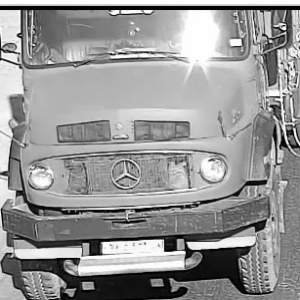
\includegraphics[width=0.9\linewidth]{../assets/gray.png}\\{\scriptsize grayscale}
    \end{center}\end{column}
    \begin{column}{0.5\textwidth}\begin{center}
      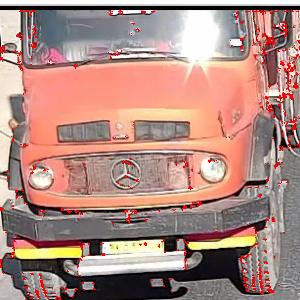
\includegraphics[width=0.9\linewidth]{../assets/harris.png}\\{\scriptsize Harris corners (red)}
    \end{center}\end{column}
  \end{columns}
  \vspace{3pt}
  Corners land on distinctive junctions (lights, edges of parts) — repeatable points to match on.
\end{frame}

\begin{frame}{The Harris algorithm, step by step}
  \begin{enumerate}
    \item Compute gradients $I_x,I_y$ (e.g.\ Sobel).
    \item Form the products $I_x^2,\ I_y^2,\ I_xI_y$ at every pixel.
    \item Smooth each product with a Gaussian window $w$ (this is the $\sum_W$).
    \item Compute $R$ per pixel from $\det$ and $\mathrm{tr}$.
    \item Threshold $R$, then apply \term{non-maximum suppression} to keep local peaks.
  \end{enumerate}
  \begin{goodbox}
    Gaussian weighting (not a box) makes the response isotropic and less noisy — the standard choice.
  \end{goodbox}
\end{frame}

\begin{frame}{Non-maximum suppression}
  \begin{columns}[T]
    \begin{column}{0.55\textwidth}
      \begin{itemize}
        \item A strong corner fires over a small blob of pixels — we want \emph{one} keypoint, not many.
        \item Keep a pixel only if its $R$ is the local maximum in a small neighbourhood.
        \item Then take the top-$N$ by score for a manageable, well-spread set.
      \end{itemize}
    \end{column}
    \begin{column}{0.45\textwidth}
      \begin{center}
      \pixelgrid{ {2,4,3}, {5,\textbf{9},6}, {3,7,4} }
      \end{center}
      {\scriptsize Center $9$ is the max of its $3{\times}3$ neighbourhood $\Rightarrow$ kept; the others are suppressed.}
    \end{column}
  \end{columns}
\end{frame}

\begin{frame}{Corner detectors}
  \begin{center}
  \begin{tabular}{@{}lll@{}}
    \toprule
    \textbf{Detector} & \textbf{Idea} & \textbf{Note} \\
    \midrule
    Harris & eigenvalues of structure matrix & classic, accurate \\
    Shi-Tomasi & min eigenvalue (goodFeaturesToTrack) & great for tracking \\
    FAST & pixel-ring intensity test & very fast, used in ORB \\
    \bottomrule
  \end{tabular}
  \end{center}
  \keyidea{Detecting \emph{where} the feature is (the keypoint) is step one. Describing \emph{what it looks like} (the descriptor) is step two.}
\end{frame}

\begin{frame}{FAST — a corner test you can do by hand}
  \begin{columns}[T]
    \begin{column}{0.52\textwidth}
      \begin{itemize}
        \item Look at a ring of 16 pixels around a candidate $p$.
        \item $p$ is a corner if $\geq 12$ contiguous ring pixels are all \emph{brighter} than
              $I_p+t$ or all \emph{darker} than $I_p-t$.
        \item A quick test of pixels 1,5,9,13 rejects most non-corners instantly.
      \end{itemize}
    \end{column}
    \begin{column}{0.48\textwidth}
      \begin{center}
      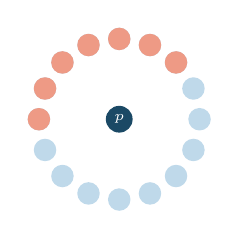
\begin{tikzpicture}[scale=0.34,font=\tiny]
        \foreach \a in {0,22.5,...,337.5}{
          \fill[courseInfo!30] (\a:3) circle (0.42);
        }
        % highlight a bright contiguous arc
        \foreach \a in {45,67.5,...,180}{
          \fill[courseAccent!70] (\a:3) circle (0.42);
        }
        \fill[coursePrimary] (0,0) circle (0.5);
        \node[white] at (0,0) {$p$};
      \end{tikzpicture}
      \end{center}
      {\scriptsize Coral arc = a contiguous run brighter than $I_p+t$.}
    \end{column}
  \end{columns}
\end{frame}

\begin{frame}{Shi-Tomasi — a small but useful tweak}
  \begin{itemize}
    \item Harris scores with $R=\lambda_1\lambda_2-k(\lambda_1+\lambda_2)^2$; Shi-Tomasi scores with
          $R=\min(\lambda_1,\lambda_2)$.
    \item A point is a good corner only if the \emph{weaker} direction is still strong — exactly what
          $\min(\lambda_1,\lambda_2)$ measures.
    \item OpenCV exposes it as \code{goodFeaturesToTrack} — the go-to for corners to \emph{track} in video.
  \end{itemize}
  \begin{infobox}[Same $M$, different score]
    Both read the structure matrix; they differ only in how they collapse its eigenvalues into one number.
  \end{infobox}
\end{frame}

\begin{frame}{Reading the gradients of a corner}
  A bright square in the lower-left of a window; its (approximate) gradient magnitudes:
  \begin{columns}[T]
    \begin{column}{0.5\textwidth}
      \begin{center}
      \pixelgrid{ {0,0,0}, {0,90,80}, {0,85,10} }
      \end{center}
      {\scriptsize Strong gradients appear along \emph{both} a vertical and a horizontal edge.}
    \end{column}
    \begin{column}{0.5\textwidth}
      \begin{itemize}
        \item Vertical edge $\rightarrow$ large $\sum I_x^2$.
        \item Horizontal edge $\rightarrow$ large $\sum I_y^2$.
        \item Both large in one window $\Rightarrow$ big $\det(M)$ $\Rightarrow$ high $R$: a corner.
      \end{itemize}
    \end{column}
  \end{columns}
  \keyidea{A corner is literally where two differently-oriented edges meet inside one window.}
\end{frame}

\begin{frame}{Choosing detector parameters}
  \begin{goodbox}
    \begin{itemize}
      \item \term{Window / $\sigma$}: larger = smoother, more stable corners but coarser localization.
      \item \term{Threshold}: set it from the score distribution (e.g.\ a fraction of the max $R$), not a magic constant.
      \item \term{Max features + NMS radius}: cap the count and spread points out for a usable, even set.
    \end{itemize}
  \end{goodbox}
  Measure success by \term{repeatability}: run the detector on the image and a warped copy, and check how
  many of the same points reappear.
\end{frame}

\begin{frame}{Pitfalls in corner detection}
  \begin{badbox}
    \begin{itemize}
      \item \term{No smoothing}: raw gradients are noisy $\rightarrow$ spurious ``corners'' on texture.
      \item \term{Wrong $k$ / threshold}: too high misses real corners; too low floods the image.
      \item \term{Skipping NMS}: you get dense clumps of near-duplicate keypoints.
    \end{itemize}
  \end{badbox}
  \keyidea{Detector quality = repeatability. Tune so the \emph{same} points reappear across views, not just ``many'' points.}
\end{frame}

% ==================================================================
\section{From keypoint to descriptor}
% ==================================================================

\begin{frame}{From keypoint to descriptor}
  \begin{itemize}
    \item A \term{descriptor} is a vector summarizing the patch around a keypoint.
    \item Good descriptors are \term{invariant}: same value under rotation, scale, and lighting change.
    \item Two images are compared by finding keypoints with \emph{similar descriptors} (next session).
  \end{itemize}
  \begin{mathbox}
    SIFT: a 128-D vector of gradient-orientation histograms; robust to rotation/scale/illumination.
  \end{mathbox}
\end{frame}

\begin{frame}{What ``invariance'' buys you}
  \begin{columns}[T]
    \begin{column}{0.5\textwidth}
      \begin{itemize}
        \item \term{Rotation}: assign the patch a dominant orientation, then describe \emph{relative} to it.
        \item \term{Scale}: describe at the feature's characteristic scale (Session 2's pyramid).
        \item \term{Illumination}: normalize the patch (subtract mean, divide by norm).
      \end{itemize}
    \end{column}
    \begin{column}{0.5\textwidth}
      \begin{center}
      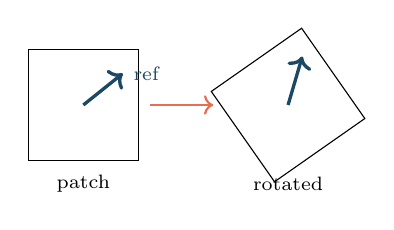
\begin{tikzpicture}[font=\scriptsize]
        \draw (0,0) rectangle (1.4,1.4);
        \draw[coursePrimary,very thick,->] (0.7,0.7)--(1.2,1.1) node[right]{ref};
        \node at (0.7,-0.3) {patch};
        \begin{scope}[xshift=2.6cm,rotate around={35:(0.7,0.7)}]
          \draw (0,0) rectangle (1.4,1.4);
          \draw[coursePrimary,very thick,->] (0.7,0.7)--(1.2,1.1);
        \end{scope}
        \node at (3.3,-0.3) {rotated};
        \draw[courseAccent,->,thick] (1.55,0.7)--(2.35,0.7);
      \end{tikzpicture}
      \end{center}
      {\scriptsize Same content, same descriptor — because we measure relative to the reference arrow.}
    \end{column}
  \end{columns}
\end{frame}

\begin{frame}{Patch normalization — a mini worked example}
  A tiny patch (before / after subtract-mean, divide-by-norm):
  \begin{columns}[T]
    \begin{column}{0.5\textwidth}
      \begin{center}
      \pixelgrid{ {10,20}, {30,40} }
      \end{center}
      {\scriptsize mean $=25$; subtract it $\rightarrow -15,-5,5,15$.}
    \end{column}
    \begin{column}{0.5\textwidth}
      \begin{center}
      \pixelgrid{ {-.6,-.2}, {.2,.6} }
      \end{center}
      {\scriptsize $\div$ norm $\approx 25.5 \rightarrow$ brightness-invariant.}
    \end{column}
  \end{columns}
  \begin{goodbox}
    A brighter copy of the same patch (add a constant, scale) normalizes to the \emph{same} vector —
    that is illumination invariance, for free.
  \end{goodbox}
\end{frame}

\begin{frame}{ORB keypoints — on the real car}
  \begin{center}
  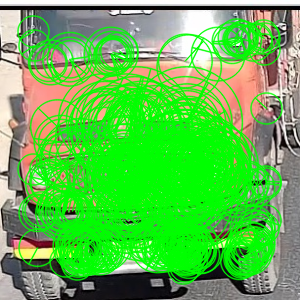
\includegraphics[width=0.5\linewidth]{../assets/orb_keypoints.png}
  \end{center}
  \begin{itemize}
    \item \term{ORB} = FAST keypoints + BRIEF descriptor, made rotation-aware (Session 2).
    \item Each circle: a keypoint with a size (scale) and orientation.
    \item $\sim$380 keypoints here — each a distinctive point ready to be described and matched.
  \end{itemize}
\end{frame}

% ==================================================================
\section{In-class exercise}
% ==================================================================

\begin{frame}{\faPen~In-class exercise (10 min)}
  \begin{infobox}[Reason about detection]
  \end{infobox}
  \begin{enumerate}
    \item Why is a corner a better feature than a point in the middle of a flat wall?
    \item A window gives $\sum I_x^2=6,\ \sum I_y^2=6,\ \sum I_xI_y=0,\ k=0.05$.
          Compute $R$. Corner, edge, or flat?
    \item You detect 5000 corners packed into clumps. Which step did you forget, and what does it fix?
  \end{enumerate}
\end{frame}

\begin{frame}{\faPen~Debrief}
  \begin{itemize}
    \item (1) A corner changes in \emph{all} directions $\rightarrow$ uniquely localizable; a flat point is ambiguous.
    \item (2) $\det=36-0=36$, $\mathrm{tr}=12$, $R=36-0.05(144)=36-7.2=\mathbf{28.8}>0 \Rightarrow$ \term{corner}.
    \item (3) \term{Non-maximum suppression} — it collapses each response blob to a single local-peak keypoint.
  \end{itemize}
  \keyidea{Detect where (Harris/FAST) $\rightarrow$ suppress duplicates $\rightarrow$ describe invariantly. Matching comes next session.}
\end{frame}

% ==================================================================
\section{Wrap-up}
% ==================================================================

\begin{frame}{What you should now be able to do}
  \begin{itemize}
    \item Explain what makes a good feature (distinctive, repeatable, local) and why corners.
    \item Derive the structure matrix and compute the Harris score $R$ by hand.
    \item Detect corners (Harris/Shi-Tomasi/FAST) and apply non-maximum suppression.
    \item Explain what a descriptor is and why invariance matters.
  \end{itemize}
\end{frame}

\begin{frame}{Next session}
  \begin{alertblock}{Session 2 — Matching \& outlier rejection}
    \begin{itemize}
      \item How SIFT and ORB actually build their descriptor vectors.
      \item Matching by Euclidean vs \term{Hamming} distance; brute-force vs FLANN.
      \item The Lowe \term{ratio test}, cross-check, and a preview of RANSAC.
      \item The week's deliverable — detect, describe, match, and filter on real images.
    \end{itemize}
  \end{alertblock}
\end{frame}

\begin{frame}[standout]
  A corner is ``a point you can find again.''\\[4pt]
  \normalsize Detect distinctive points, suppress duplicates, and get them ready to describe.
\end{frame}

\end{document}
